\chapter{Proposta}
\label{capitulo_proposta}
Os atrasos existentes em equipamentos elétricos utilizados em redes ópticas têm diversas origens, como o processamento dos dados (intrinsecamente relacionado ao poder de processamento do equipamento) e as conversões de meio necessárias, sendo que para cada equipamento pode-se considerar pelo menos duas dessas conversões (óptica-elétrica-óptica). 

Logo, todas as vezes que um pacote trafega em uma rede óptica acaba sofrendo atrasos, que são traduzidos em forma de latência, em cada um dos nós participantes do circuito. Estes atrasos devem ser somados a fim de determinar a latência total de um enlace. A Figura \ref{fig_latency_link} mostra a acúmulo da latência através de um enlace óptico entre dois pontos. 

\begin{figure} [!htb]% normalmente utilizar [!t]
	\centering
	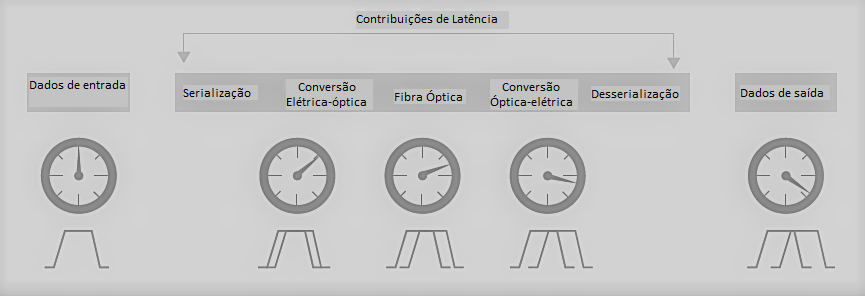
\includegraphics[width=1\textwidth]{./figuras/latency-link.png}
	\caption[Latência de Link]{Latência em comunicação entre dois pontos utilizando link óptico. Os principais pontos de inserção de latência na comunicação são resultantes dos processos de conversão elétrica-óptica, transmissão de dados, conversão óptica-elétrica e disponibilização dos dados no destino (desserialização e processamento).}
	\fonte{\cite{Art-Coffe2017}}
	\label{fig_latency_link}
\end{figure}

Logo, a proposta apresentada neste artigo, denominada de \sigla{BSN}{\emph{``Bypass Seletivo de Nós''}} \emph{``Bypass Seletivo de Nós''}, ocupa um lugar intermediário entre os equipamentos puramente ópticos e os ópticos/elétricos. Conforme descrito na seção \ref{cap_protocolos_de_roteamento} um protocolo de roteamento é responsável pelo tratamento e pela dinâmica das mensagens e dados trocados entre os dispositivos participantes da comunicação. Como dinâmica pode-se citar o cálculo de rotas a serem utilizadas e, desta forma pode-se configurar o BSN como um protocolo especificamente desenvolvido para otimização de latência em redes ópticas através da utilização de chaveadores ópticos em pontos estratégicos da rede, ou seja, através da manipulação do \emph{layer} físico da rede. Dessa forma equipamentos em posições específicas da rede podem ser desviados sem a necessidade de nenhuma conversão de meio ou mesmo processamento, resultando na mínima inserção de latência possível. 

O BSN opera de maneira completamente desagregada do protocolo de roteamento utilizado na rede em questão. Ele pode ser utilizado em qualquer rede que contenha multi-caminhos ou redundâncias de maneira a possibilitar a criação de novas topologias a partir da reorganização das ligações físicas. Para tanto, é necessário que a rede em questão possa ser representada por um grafo simples, ou seja, um grafo que não possui arestas paralelas ou pontas coincidentes (laços) conforme anteriormente descrito em \ref{chap_grafos}.

Os pontos da rede de acionamento do chaveador óptico podem ser escolhidos em ramos de um grafo com muitos vértices (\emph{hops}) ou podem ser planejados para o estabelecimento de rotas específicas para comunicação com pontos críticos do sistema, estabelecendo um \sigla{SLA}{\emph{Service Level Agreement}} em \emph{layer} físico.

Através da utilização do BSN é possível reduzir o grafo da rede possibilitando uma nova configuração de conexões inexistente na rede original e consequentemente uma nova variedade de rotas possíveis. Cada vez que o BSN ativa um \emph{bypass}, as duas arestas envolvidas são unificadas evitando o vértice das mesmas, criando assim um novo grafo com uma distância entre os dois vértices finais de um vértice a menos, como representado na Figura \ref{fig-bypass-exemplo}. Dessa forma, em caso de falha ou mudança de SLA, a topologia física pode ser alterada automaticamente.

\begin{figure}[t!]
	\centering
	\begin{subfigure}[t]{0.4\textwidth}
		\centering
		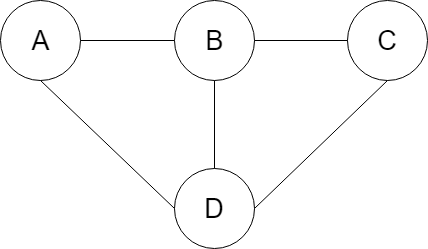
\includegraphics[width=4cm]{./figuras/Bypass-exemplo-A.png} % <- formatos PNG, JPG e PDF
		\caption{Chaveador óptico desativado}
		\label{fig_bypass_exemplo_A}
	\end{subfigure}%
	~
	\begin{subfigure}[t]{0.4\textwidth}
		\centering
		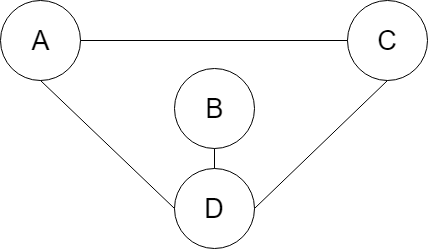
\includegraphics[width=4cm]{./figuras/Bypass-exemplo-B.png} % <- formatos PNG, JPG e PDF
	\caption{Chaveador óptico ativado}
	\label{fig_bypass_exemplo_B}
	\end{subfigure}
	\caption[Exemplo de atuação de \emph{by-pass} óptico]{Efeito da utilização do chaveador ótico em uma rede de comunicação. Em \ref{fig_bypass_exemplo_A} pode-se ver a rede original contendo dois saltos entre os vértices A e C. Em \ref{fig_bypass_exemplo_B} após o acionamento do dispositivo no vértice B pode-se ver e existência de apenas um salto entre os vértices A e C}
	\label{fig-bypass-exemplo}
\end{figure}

\section{BSN}
Esta seção descreve o funcionamento da proposta através de um exemplo simplificado, discorre sobre a implementação do algoritmo utilizado para criação do BSN assim como sobre a ferramenta criada para simulações e criação dos dados utilizados no presente estudo.

\subsection{Funcionamento do BSN}
Para exemplificar o funcionamento do BSN foi gerada a rede da Figura \ref{BSN-example-network}. Essa rede foi gerada pelo software desenvolvido para avaliação do BSN, posteriormente descrito de maneira detalhada na Seção \ref{implementacao}. Como pode-ser notar essa rede é representada por um grafo simples com valência igual a 3, e pode ser classificada de acordo com o exposto na Seção \ref{redes-de-computadores} com sendo uma rede \emph{mesh}. 

O grafo da Figura \ref{BSN-example-network} foi submetido ao software de simulação para cálculo dos caminhos ótimos para todos os vértices à partir do vértice origem (arbitrariamente escolhido como sendo o 1) e a Figura \ref{BSN-example-network-tree} mostra o resultado desta operação. Esta figura representa os caminhos ótimos para, saindo do vértice raiz, alcançar todos os demais vértices. Deste modo, grafo da Figura \ref{BSN-example-network} representa o melhor caso possível em termos de profundidade de rede.

Após as melhores rotas terem sido descobertas conforme descrito, a rede da Figura \ref{BSN-example-network} foi submetida ao software de simulação para a execução do BSN. Como resultado decidiu-se pelo acionamento do chaveador óptico no vértice 7, interligando o vértice 1 diretamente ao 4 gerando um novo grafo da rede conforme representado na Figura \ref{BSN-example-opt-switch}. Este grafo, quando submetido ao cálculo dos caminhos ótimos, assim como realizado com a rede original, resulta no grafo da Figura \ref{BSN-example-rede-otimizada}, onde pode-se notar a diminuição da profundidade em comparação com aquele mostrado na Figura \ref{BSN-example-network-tree}.

\begin{figure}[t!]
	\centering
	\begin{subfigure}[t]{0.4\textwidth}
		\centering
		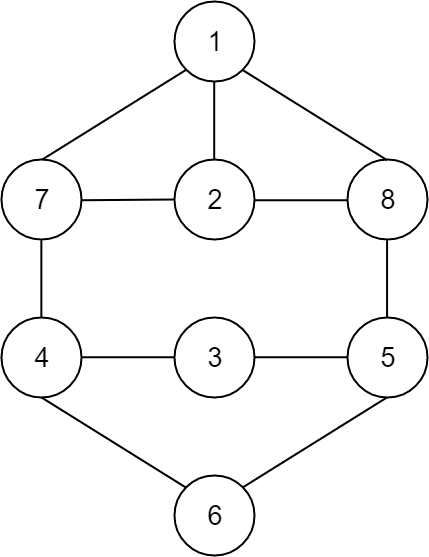
\includegraphics[width=4cm]{./figuras/BSN-ex-network-generation.png} % <- formatos PNG, JPG e PDF
		\caption{Rede gerada}
		\label{BSN-example-network}
	\end{subfigure}%
	~
	\begin{subfigure}[t]{0.4\textwidth}
		\centering
		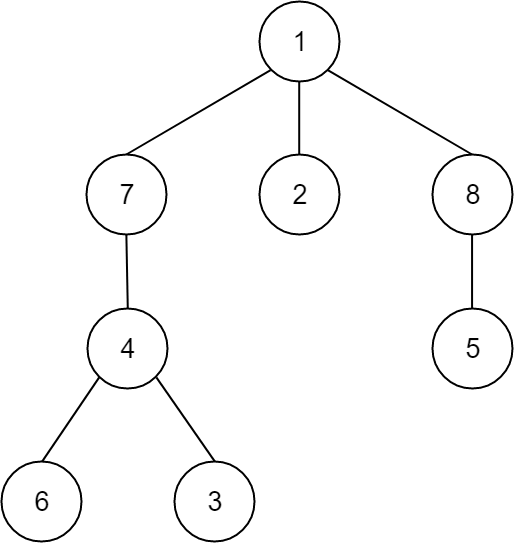
\includegraphics[width=4cm]{./figuras/BSN-ex-network-generation-tree.png} % <- formatos PNG, JPG e PDF
	\caption{Árvore da Rede}
	\label{BSN-example-network-tree}
	\end{subfigure}
	~
	\begin{subfigure}[t]{0.4\textwidth}
		\centering
		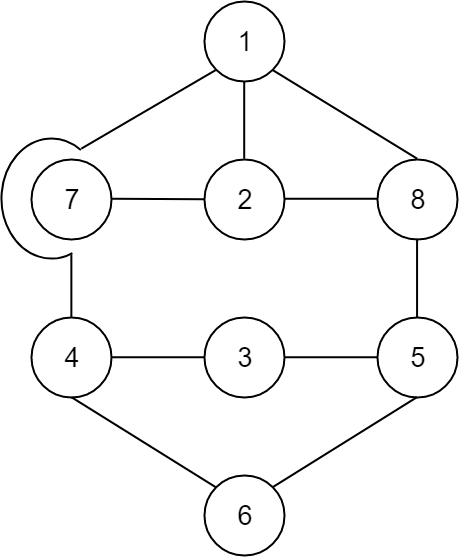
\includegraphics[width=4cm]{./figuras/BSN-ex-bypass.png} % <- formatos PNG, JPG e PDF
	\caption{Chaveador óptico ativado}
	\label{BSN-example-opt-switch}
	\end{subfigure}
	~
	\begin{subfigure}[t]{0.4\textwidth}
		\centering
		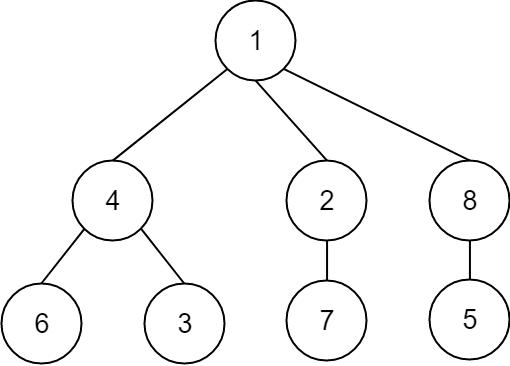
\includegraphics[width=4cm]{./figuras/BSN-ex-network-final.png} % <- formatos PNG, JPG e PDF
	\caption{Rede resultante}
	\label{BSN-example-rede-otimizada}
	\end{subfigure}
	\caption[Exemplo de funcionamento do BSN]{Exemplo de funcionamento do protocolo BSN. Percebe-se que o BSN consegue reduzir a profundidade de uma rede gerando uma nova possibilidade de conexões através da manipulação da camada física da mesma.}
	\label{fig-bsn-exemplo}
\end{figure}

Este exemplo ilustra, em uma rede de apenas 8 nós, o funcionamento do protocolo proposto (BSN). É possível notar que a profundidade da rede, ligada à latência da comunicação, é reduzida impactando na redução de latência para a comunicação entre os nós envolvidos.

\subsection{Implementação}
\label{implementacao}
O método de redução do grafo de rede utilizado pelo BSN é descrito sucintamente em alto nível através do pseudocódigo representado no Algoritmo \ref{pseudocode_bsn}. O BSN utiliza vários conceitos de otimização simultâneos. A ideia básica é a utilização de um algoritmo genético para a criação de diferentes combinações de estado dos chaveadores ópticos na rede (de acordo com as premissas de projeto a serem adotadas). Dessa forma, cada uma das combinações geradas pelo algoritmo genético acaba por gerar uma nova topologia de conexões físicas, que são por sua vez otimizadas buscando obter a rede menos profunda possível. 

Esta busca compreende, em essência, a escolha de quais arestas do grafo serão utilizadas para estabelecer a comunicação entre os nós e quais não serão utilizadas. Dessa forma, para o passo representado na linha \ref{bsn:fitness_line} do Algoritmo \ref{pseudocode_bsn} (busca local), que representa exatamente este passo do código, pode ser utilizado qualquer algoritmo conhecido. Daí vem o fato de o BSN ter a capacidade de ser utilizado com qualquer protocolo padrão de otimização de rede como o STP por exemplo. O presente documento utiliza para este passo uma busca de custo uniforme, garantindo assim a obtenção do valor ótimo de \emph{fitness}, que neste código está relacionado ao custo total da rede. Ou seja, o algoritmo de custo uniforme irá resultar na melhor rede possível para o grafo em questão já que este tipo de busca é exaustiva e explora todas as combinações possíveis para então selecionar a melhor delas.

\begin{algorithm} [h]
\caption{ - Algoritmo básico do BSN}
\begin{algorithmic}[1]
\State $popsize\gets \textit{tamanho da populacao}$
\State $gennumb\gets \textit{numero de geracoes}$\\
\State PopList[] = new List[popsize]\Comment{Variável para alocação da geração atual}
\State $i\gets 0$
\While {$ i< popsize $}
\State Individuo = CriaIndividuo()\Comment{Cria a uma configuração de rede}
\State CalculaFit(Individuo)\label{bsn:fitness_line}\Comment{Realiza busca local na instância de rede}
\State PopList.Add(Individuo)\Comment{Adiciona a instância de rede à lista}
\State PopList.ClassifcaIndividuos()\Comment{Organiza a população atual de acordo com o Fitness individual}
\EndWhile\Comment{População inicial criada}\\
\State $j\gets 1$
\While {$ j< gennumb $}\Comment{Roda algoritmo genético}
\State ParentsList[] = new List[]\Comment{Variável para alocação de indivíduos ``pais''}
\State NewList[] = new List[popsize]\Comment{Variável para alocação de próxima geração}
\State ParentsList = SelecionaIndividuos(PopList)\Comment{Seleciona os indivíduos da geração atual que serão utilizados para criação da geração seguinte}
\State NewList = CrossOver(ParentsList)\Comment{Cruza os indivíduos selecionados}
\State Mutation(NewList)\Comment{Aplica algoritmo de mutação de genes na nova população}
\State PopList = MesclaGen(NewList, PopList)\Comment{Realiza elitismo de indivíduos}
\State PopList.ClassifcaIndividuos()\Comment{Organiza a população atual de acordo com o Fitness individual}
\EndWhile\\
\State\Return PopList.Individuo(0)\Comment{Retorna melhor instância de rede}
\end{algorithmic}
\label{pseudocode_bsn}
\end{algorithm}

\subsubsection{Custo da rede}
\label{subsection-custo-da-rede}
O custo da rede é definido como a soma de todos os custos individuais (número de saltos) para comunicação em cada um dos \emph{links} da rede. Logo, utilizando a rede de exemplo representada na Figura \ref{BSN-example-network-tree} tem-se o mostrado na Tabela \ref{tab-custo-rede-BSN-example-network-tree} como sendo os custos individuais para comunicação entre o nó origem e os demais assim como o custo total da rede. Em contrapartida, ao utilizar a rede representada na Figura \ref{BSN-example-rede-otimizada}, que foi otimizada através da utilização do BSN, tem-se como resultado para os custos individuais e custo total o representado na Tabela \ref{tab-custo-rede-bsn-otimizada}.

A partir da comparação dos dados apresentados na Tabela \ref{tab_calc_custo} nota-se que o custo total da rede foi otimizado em aproximadamente 15,4\% (o que por si só já representa um grande ganho) mas, além disso, ao comparar o custo de cada um dos nós de maneira individual pode-se notar que para os destinos 3 e 6 foi alcançado 33,33\% de melhoria e para os destinos 4 e 7 foi alcançado 50\% de melhoria.

Assim fica claro o BSN não apenas minimiza o custo ou latência da rede como um todo mas apresenta, em especial, um ótimo resultado ao avaliar-se o custo de uma rota em específico. Desta forma o protocolo proposto pode ser extremamente útil no estabelecimento de políticas de \sigla{QoS}{\emph{Quality of Service}} em layer físico, sendo esta uma aplicação jamais explorada anteriormente.

\setcounter{table}{1} \renewcommand{\thetable}{\arabic{table}}
\begin{table}[t!]
	\centering
	\begin{subfigure}[t]{0.4\textwidth}
		\centering
		%\begin{table}[]
			\begin{tabular}{llllll}
			\hline
			\multicolumn{1}{|l|}{\textbf{Nó destino}} & \multicolumn{4}{c}{\textbf{Caminho}} & \multicolumn{1}{c|}{\textbf{Custo}} \\ \hline
			\multicolumn{1}{|l|}{\textbf{2:}} & 1 & 2 &  & \multicolumn{1}{l|}{} & \multicolumn{1}{l|}{1} \\ \hline
			\multicolumn{1}{|l|}{\textbf{3:}} & 1 & 7 & 4 & \multicolumn{1}{l|}{3} & \multicolumn{1}{l|}{3} \\ \hline
			\multicolumn{1}{|l|}{\textbf{4:}} & 1 & 7 & 4 & \multicolumn{1}{l|}{} & \multicolumn{1}{l|}{2} \\ \hline
			\multicolumn{1}{|l|}{\textbf{5:}} & 1 & 8 & 5 & \multicolumn{1}{l|}{} & \multicolumn{1}{l|}{2} \\ \hline
			\multicolumn{1}{|l|}{\textbf{6:}} & 1 & 7 & 4 & \multicolumn{1}{l|}{6} & \multicolumn{1}{l|}{3} \\ \hline
			\multicolumn{1}{|l|}{\textbf{7:}} & 1 & 7 &  & \multicolumn{1}{l|}{} & \multicolumn{1}{l|}{1} \\ \hline
			\multicolumn{1}{|l|}{\textbf{8:}} & 1 & 8 &  & \multicolumn{1}{l|}{} & \multicolumn{1}{l|}{1} \\ \hline
			 & \multicolumn{4}{l}{\textbf{Custo Total}} & \textbf{13}
			\end{tabular}
		\caption{Calculo de custo - Rede Figura \ref{BSN-example-network-tree}}
		\label{tab-custo-rede-BSN-example-network-tree}
		%\end{table}
	\end{subfigure}%
	~
	\begin{subfigure}[t]{0.4\textwidth}
		\centering
			%\begin{table}[]
			\begin{tabular}{lllll}
			\hline
			\multicolumn{1}{|l|}{\textbf{Nó destino}} & \multicolumn{3}{c}{\textbf{Caminho}} & \multicolumn{1}{c|}{\textbf{Custo}} \\ \hline
			\multicolumn{1}{|l|}{\textbf{2:}} & 1 & 2 & \multicolumn{1}{l|}{} & \multicolumn{1}{l|}{1} \\ \hline
			\multicolumn{1}{|l|}{\textbf{3:}} & 1 & 4 & \multicolumn{1}{l|}{3} & \multicolumn{1}{l|}{2} \\ \hline
			\multicolumn{1}{|l|}{\textbf{4:}} & 1 & 4 & \multicolumn{1}{l|}{} & \multicolumn{1}{l|}{1} \\ \hline
			\multicolumn{1}{|l|}{\textbf{5:}} & 1 & 8 & \multicolumn{1}{l|}{5} & \multicolumn{1}{l|}{2} \\ \hline
			\multicolumn{1}{|l|}{\textbf{6:}} & 1 & 4 & \multicolumn{1}{l|}{6} & \multicolumn{1}{l|}{2} \\ \hline
			\multicolumn{1}{|l|}{\textbf{7:}} & 1 & 2 & \multicolumn{1}{l|}{7} & \multicolumn{1}{l|}{2} \\ \hline
			\multicolumn{1}{|l|}{\textbf{8:}} & 1 & 8 & \multicolumn{1}{l|}{} & \multicolumn{1}{l|}{1} \\ \hline
			 & \multicolumn{3}{l}{\textbf{Custo Total}} & \textbf{11}
			\end{tabular}
	\caption{Calculo de custo - Rede Figura \ref{BSN-example-rede-otimizada}}
	\label{tab-custo-rede-bsn-otimizada}
	%\end{table}
	\end{subfigure}
	\caption[Exemplo de cálculo de custo total em rede]{Exemplificação do cálculo e comparação entre o custo total para duas redes exemplo}
	\label{tab_calc_custo}
\end{table}

\subsubsection{Representação - VERIFICAR ESTE TITULO}
Na Computação Evolutiva de maneira geral é comum encontrar de termos da biologia para representar estruturas e variáveis, o mesmo acontece no campo dos AGs, como no caso do BSN. No presente documento a relação entre estes termos é dada conforme o mostrado na Tabela \ref{tab-correlacao-bio-comp}.

\begin{table}[ht]
\centering
\begin{tabular}{|l|l|}
\hline
\multicolumn{1}{|c|}{\textbf{Biologia}} & \multicolumn{1}{c|}{\textbf{Computação}} \\ \hline
Cromossomo & Indivíduo \\ \hline
Gene & Caractere \\ \hline
Alelo & Valor do caractere \\ \hline
Lócus & Posição do caractere \\ \hline
Genótipo & Vetor de caracteres representando o indivíduo \\ \hline
Fenótipo & Interpretação do vetor de caracteres \\ \hline
\end{tabular}
\caption[Biologia x BSN]{Correlação entre vocábulos da Biologia e os utilizados no BSN}
\label{tab-correlacao-bio-comp}
\end{table}  

Seguindo estas definições, o BSN cria um conjunto de Cromossomos, denominado de população. Esta população é constituída pelos diversos indivíduos cujos Genótipos estão baseados na rede em questão. Cada um dos Cromossomos é representado como sendo um vetor \emph{booleano} com o número de Genes igual ao número de nós da rede a ser otimizada e onde cada um dos Lócus representa unicamente um nó. Os Alelos por sua vez representam o estado do chaveador ótico no respectivo nó. Em resumo, seguindo esta convenção, pode-se representar a rede mostrada na Figura \ref{BSN-example-opt-switch} através do Cromossomo (ou indivíduo) da Tabela \ref{tab-cromossomo-bsn}.

\begin{table}[ht]
\centering
\begin{tabular}{|l|l|l|l|l|l|l|l|l|}
\hline
\multicolumn{1}{|c|}{\textbf{Nó}} & \multicolumn{1}{c|}{1} & 2 & 3 & 4 & 5 & 6 & 7 & 8 \\ \hline
\textbf{Cromossomo} & 0 & 0 & 0 & 0 & 0 & 0 & 1 & 0 \\ \hline
\end{tabular}
\caption[Cromossomo BSN]{Repesentação da estrutura básica de um cromossomo do BSN}
\label{tab-cromossomo-bsn}
\end{table}

Como pode-se notar cada um dos Lócus do Cromossomo representa um nó da rede, logo tem-se um Cromossomo com 8 Genes visto que a rede tem 8 nós, além disso o Alelo do Lócus 7 é igual a 1, o que pode ser interpretado como a informação de que o chaveador óptico instalado no nó 7 está ligado enquanto os outros estão desligados (Alelos 0). Dessa forma, o Fenótipo deste indivíduo, ou seja, a interpretação deste Cromossomo, indica que o grafo desta rede deve ser representado considerando que o chaveador óptico referente ao nó 7 está acionado e os demais não, como representado na Figura \ref{BSN-example-opt-switch}.

\subsubsection{Função de \emph{Fitness}}
Como em qualquer AG o BSN baseia seu funcionamento na avaliação de uma função de \emph{fitness}, que conforme brevemente descrito na Seção \ref{implementacao} está atrelada ao custo da rede. De maneira geral, o custo total da rede é calculado conforme descrito em \ref{subsection-custo-da-rede}, com a diferença da necessidade de adoção de uma convenção em caso da avaliação de um grafo desconexo.

Basicamente, a utilização do BSN pode gerar redes específicas onde nem todos os nós sejam acessíveis devido ao acionamento do chaveador óptico em posições inadequadas. Em outras palavras, podem existir Genótipos que dêem origem a redes cujos grafos são desconexos como o da Figura \ref{fig_grafo_desconexo}. Neste caso o custo dessa rede, de acordo com o descrito em \ref{subsection-custo-da-rede} seria infinito, visto que o custo unitário para alcançar o(s) vértice(s) não conectado(s) seria infinito. Logo necessita-se de uma convenção para representar este custo visto que ``infinito'' não pode ser representado computacionalmente. Adotou-se que o custo de um link como o descrito é igual a 1000 (mil unidades de custo), dessa forma o custo total da rede deverá seguir a Equação \ref{eq-fitness}. Como consequência o custo da rede deverá conter uma parcela múltipla de 1000 no caso em que existam um ou mais nós sem conexão com o nó origem. 

\setcounter{equation}{0} \renewcommand{\theequation}{\arabic{equation}}
\begin{equation}
\begin{split}
Fitness_{BSN} = \sum_{n=1}^{x}custo_{1}(n) \rightarrow custo_{orig}(dst)=\left\{\begin{matrix}
h.p, \textup{para nó conectado}\\ 1000, \textup{para nó desconectado}
\end{matrix}\right.
\\onde:\\
x=\textup{número de nós}
\\orig=\textup{vértice origem}
\\dst=\textup{vértice destino}
\\h=\textup{número de \emph{hops} entre orig e dst}
\\p=\textup{peso do \emph{hop} em questão (custo do link)}
\end{split}
\label{eq-fitness}
\end{equation}

\subsubsection{\emph{Crossover}}
O processo de \emph{Crossover} é o responsável pela criação de novos indivíduos, também chamados de filhos, que serão constituintes da nova geração. Existem muitos métodos diferentes que podem ser utilizados para esta operação, a Figura \ref{fig_crossover} exemplifica o método de \emph{Crossover} simples já que este foi o escolhido no BSN.

\begin{figure} [!htb]% normalmente utilizar [!t]
	\centering
	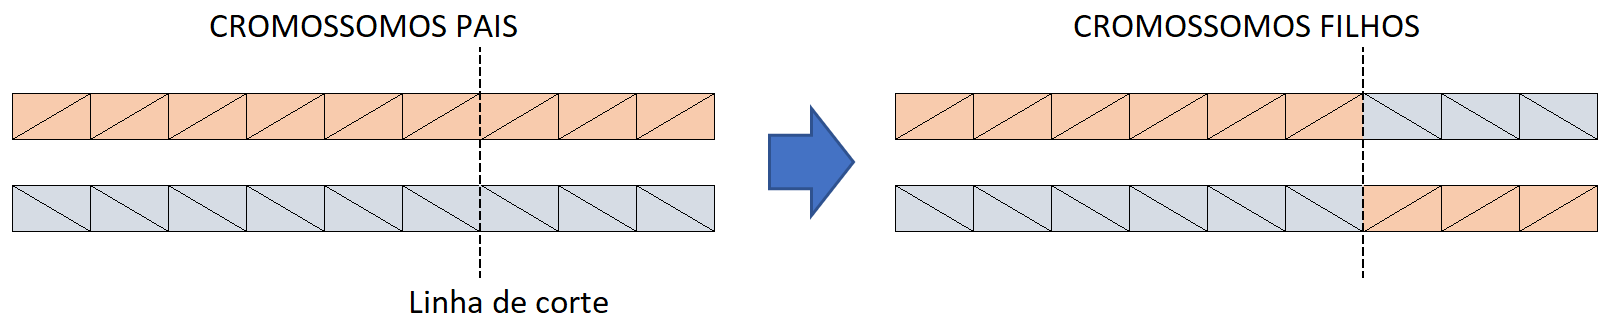
\includegraphics[width=1\textwidth]{./figuras/crossover.png}
	\caption[Exemplo de \emph{Crossover}]{Exemplo de operação de \emph{Crossover} Simples.}
	\label{fig_crossover}
\end{figure}

Como pode-se notar dois cromossomos pais são escolhidos e um ponto de corte é definido de maneira aleatória, os cromossomos são então divididos neste ponto de corte e recriados através da troca de informações entre si. Desta forma os cromossomos filhos são gerados através do compartilhamento de informação genética dos pais, criando um novo indivíduo com um novo valor de \emph{fitness}.

\subsubsection{Seleção}
Paralelamente à Seleção Natural, os AGs utilizam-se de diferentes recursos para selecionar os indivíduos de cada geração mais adaptados ao problema em questão. O BSN utiliza o conceito de \emph{``Roulette Wheel''} \cite{Goldberg1889}. 

Neste tipo de seleção toda a população é avaliada de maneira a criar uma correlação percentual entre o valor de \emph{fitness} de cada um dos indivíduos e sua representatividade perante toda a população. Desse modo pode-se ter um indicativo de quão adaptado cada um deles é com relação a sua geração corrente, e então é possível criar uma distribuição de probabilidades para a escolha de cada um dos mesmos no processo de reprodução.

Seguindo esse critério os pais, que irão fornecer o código genético para a nova geração, deverão potencialmente ser os mais adaptados ao problema em questão aumentando a chance de criar descendentes ainda mais adaptados e, desta forma, acelerando a convergência do algoritmo. A Tabela \ref{tab-selecao} exemplifica este critério de seleção, conforme pode-se ver o indivíduo $\beta$ possui um \emph{fitness} que corresponde a um índice de adaptabilidade ao problema proposto de 43,44\%, logo ele possui 44,33\% de chances de ser escolhido para reprodução enquanto o indivíduo $\alpha$ possui apenas 11,33\% de chance de ser escolhido.

\begin{table}[ht]
\centering
\begin{tabular}{|l|l|l|}
\hline
\multicolumn{1}{|c|}{\textbf{Indivíduo}} & \multicolumn{1}{c|}{\textbf{\emph{Fitness}}} & \textbf{Percentual do Total} \\ \hline
\textbf{$\alpha$} & 34 & 11,33\% \\ \hline
\textbf{$\beta$} & 130 & 43,33\% \\ \hline
\textbf{$\delta$} & 66 & 22\% \\ \hline
\textbf{$\theta$} & 70 & 23,33 \\ \hline
\textbf{Total} & \textbf{300} & \textbf{100\%} \\ \hline
\end{tabular}
\caption[\emph{``Roulette Wheel''}]{Exemplo de aplicação do Método de Seleção \emph{``Roulette Wheel''}}
\label{tab-selecao}
\end{table}

\subsubsection{Dimensão das Populações}
O sucesso de qualquer AG está intrinsecamente relacionado ao tamanho de sua população inicial e das subsequentes gerações. Caso a quantidade de indivíduos em cada uma delas seja muito grande ou muito pequena a evolução dos mesmos pode ser comprometida. Segundo \cite{Goldberg1889} estes parâmetros devem ser estabelecidos empiricamente baseados na disponibilidade dos recursos computacionais utilizados.

Para as simulações do BSN foram utilizadas populações de 500 indivíduos, este valor mostrou-se suficiente para alcançar valores ótimos de custo em várias redes de teste e foi adotado como padrão para as simulações posteriormente descritas.

\subsubsection{Parâmetros Adotados}
Para a utilização do BSN, assim como em qualquer AG, alguns parâmetros básicos precisam ser configurados. A Tabela \ref{tab-parametros} mostra os parâmetros utilizados nas simulações do BSN apresentadas na Seção \ref{resultados}.

\begin{table}[ht]
\centering
\begin{tabular}{|l|l|l|l|l|}
\hline
\multicolumn{1}{|c|}{\textbf{\begin{tabular}[c]{@{}c@{}}Tamanho da \\ População\end{tabular}}} & \multicolumn{1}{c|}{\textbf{\begin{tabular}[c]{@{}c@{}}Número de \\ Gerações\end{tabular}}} & \multicolumn{1}{c|}{\textbf{\begin{tabular}[c]{@{}c@{}}Método de escolha\\ de indivíduo para \\ reprodução\end{tabular}}} & \multicolumn{1}{c|}{\textbf{\begin{tabular}[c]{@{}c@{}}Probabilidade de \\ \emph{Crossover}\end{tabular}}} & \multicolumn{1}{c|}{\textbf{\begin{tabular}[c]{@{}c@{}}Probabilidade de \\ Mutação\end{tabular}}} \\ \hline
500 & 50 & \emph{Roulette Wheel} & 94\% & 0,5\% \\ \hline
\end{tabular}
\caption[Parâmetros do BSN]{Parâmetros básicos utilizados no algoritmo do BSN}
\label{tab-parametros}
\end{table}


\subsection{programa de simulação}

\section{Resultados}
\label{resultados}